\documentclass{beamer}

\setbeamertemplate{footline}[text line]{%
\parbox{\linewidth}{\vspace*{-8pt}29/3/23\hfill Department of Information Technology \hfill\insertpagenumber}}
\setbeamertemplate{navigation symbols}{}
\usepackage{graphicx}
\usepackage[sfdefault]{carlito}
%\usefonttheme{serif}
\usepackage{tabularx}
\usepackage{bookman}
\usepackage{fancyhdr}
\usepackage{xcolor}
\usepackage{hyperref}

\usepackage[T1]{fontenc}[12pt]
\usecolortheme{orchid}
\beamertemplateballitem
\usepackage{ragged2e}
\apptocmd{\frame}{}{\justifying}{}
\begin{document}

\begin{frame}
\begin{picture}(-3,-3)
\put(-22,0){
\includegraphics[width=40pt,height=50pt]{logo.png}}
\put(90,25){\textbf{\LARGE BVRIT HYDERABAD}}
\newline \put(80,10){\large College of Engineering for Women }
\put(298,-10){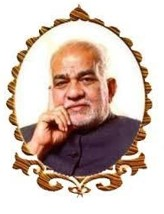
\includegraphics[width=40pt,height=60pt]{bvraju.png}}
\end{picture}
\put(60,-50){\textbf{{\LARGE  PRODUCT CLASSIFICATION 2} }}
\put(180,-115){{\normalsize Team No: 9}}
\put(180,-130){Team Members:}
\put(180,-150){A.Swetha-20WH1A12A4}
\put(180,-159){B.Saisree-20WH1A12A5}
\put(180,-169){K.Akhila-20WH1A12A6}
\put(180,-179){B.Gouthami-20WH1A12A7}
\put(180,-189){P.Meghana-20WH1A12A8}
\end{frame}

\begin{frame}
\frametitle{
\begin{picture}(-3,-3)
\put(-10,-30){
\includegraphics[width=40pt,height=50pt]{logo.png}}
\end{picture}
\put(110,-20){\color{black}\textbf {TABLE OF CONTENTS}}
\begin{picture}(-3,-3)
\put(315,-40){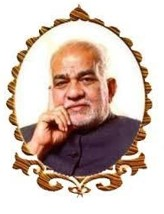
\includegraphics[width=40pt,height=60pt]{bvraju.png}}
\end{picture}}


\begin{itemize}
\item Problem statement
\item Python Packages used
\item Algorithm
\item Output
\item Comparison table
\end{itemize}
\end{frame}


\begin{frame}
\frametitle{
\begin{picture}(-3,-3)
\put(-10,-30){
\includegraphics[width=40pt,height=50pt]{logo.png}}
\end{picture}
\put(110,-20){\color{black}\textbf {Problem Statement}}
\begin{picture}(-3,-3)
\put(315,-40){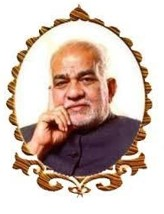
\includegraphics[width=40pt,height=60pt]{bvraju.png}}
\end{picture}}
\justifying
\begin{itemize}
\item
Each row in the dataset has been labeled with one
true Class. For each row submit the predicted
probabilities that the product belongs to each class
label. Submissions are evaluated using multi-class
logarithmic loss.
\end{itemize}
\begin{figure}
{
\includegraphics[width=6cm,height=2cm]{logloss.png}}
\end{figure}


\end{frame}



\begin{frame}
\frametitle{
\begin{picture}(-3,-3)
\put(-10,-30){
\includegraphics[width=40pt,height=50pt]{logo.png}}
\end{picture}
\put(110,-20){\color{black}\textbf {Python Packages Used}}
\begin{picture}(-3,-3)
\put(315,-40){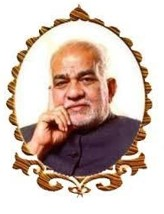
\includegraphics[width=40pt,height=60pt]{bvraju.png}}
\end{picture}}
\justifying
\begin{itemize}
\item Numpy 
\item Pandas 
\item Label encoder
\item sklearn 

\end{itemize}
\end{frame}

\begin{frame}
\frametitle{
\begin{picture}(-3,-3)
\put(-10,-30){
\includegraphics[width=40pt,height=50pt]{logo.png}}
\end{picture}
\put(110,-20){\color{black}\textbf {Algorithm}}
\begin{picture}(-3,-3)
\put(315,-40){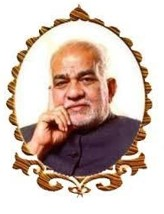
\includegraphics[width=40pt,height=60pt]{bvraju.png}}
\end{picture}}
\justifying
\begin{itemize}
\item Multinomial Logistic Regression.
\item XGBoost
\item Random Forest Classifier.
\end{itemize}
\end{frame}
\begin{frame}
\frametitle{
\begin{picture}(-3,-3)
\put(-10,-30){
\includegraphics[width=40pt,height=50pt]{logo.png}}
\end{picture}
\put(135,-20){\color{black}\textbf{Output}}
\begin{picture}(-3,-3)
\put(315,-40){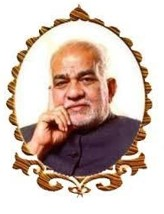
\includegraphics[width=40pt,height=60pt]{bvraju.png}}
\end{picture}}
\begin{itemize}
\item RANDOM FOREST CLASSIFIER
\end{itemize}
\begin{figure}
{\includegraphics[width=8cm,height=4cm]{randomforest.png}}
\end{figure}

\end{frame}




\begin{frame}
\frametitle{
\begin{picture}(-3,-3)
\put(-10,-30){
\includegraphics[width=40pt,height=50pt]{logo.png}}
\end{picture}
\put(135,-20){\color{black}\textbf{Output}}
\begin{picture}(-3,-3)
\put(315,-40){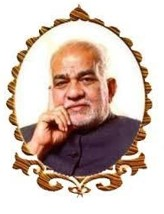
\includegraphics[width=40pt,height=60pt]{bvraju.png}}
\end{picture}}
\begin{itemize}
\item XGBOOST
\end{itemize}
\begin{figure}
{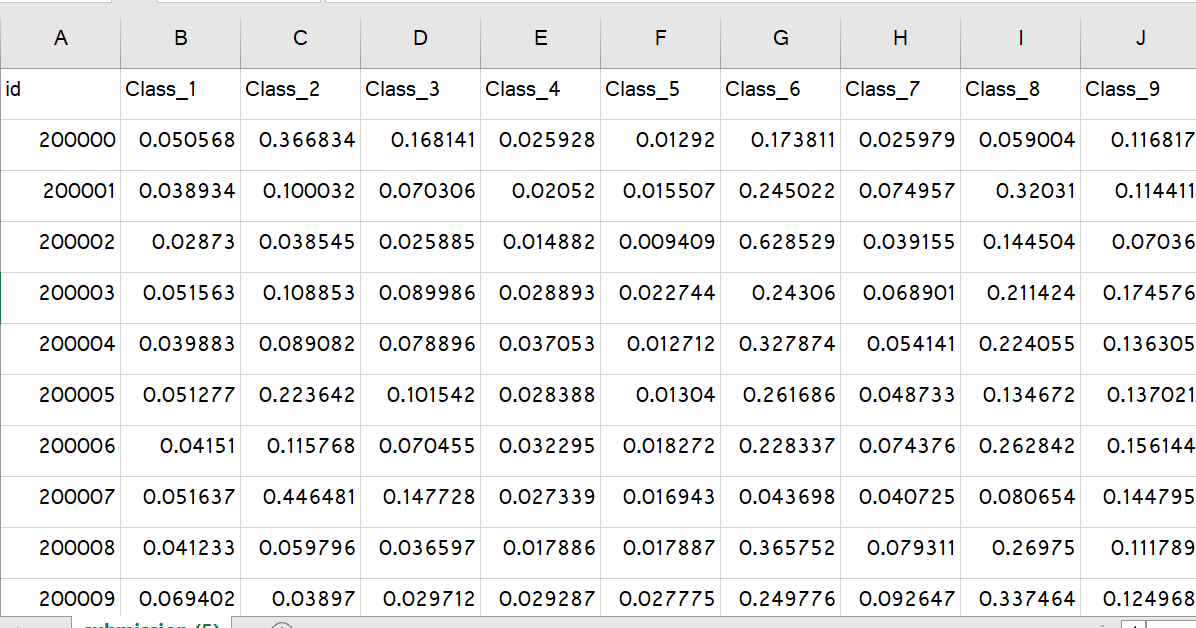
\includegraphics[width=8cm,height=4cm]{xgboost.png}}
\end{figure}

\end{frame}




\begin{frame}
\frametitle{
\begin{picture}(-3,-3)
\put(-10,-30){
\includegraphics[width=40pt,height=50pt]{logo.png}}
\end{picture}
\put(125,-20){\color{black}\textbf{Comparison Table}}
\begin{picture}(-3,-3)
\put(315,-40){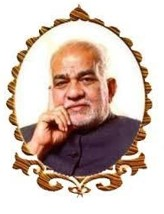
\includegraphics[width=40pt,height=60pt]{bvraju.png}}
\end{picture}}
\begin{figure}
{\includegraphics[width=8cm,height=6cm]{compare.png}}
\end{figure}

\end{frame}





\begin{frame}

\begin{center}
\frametitle{
\begin{picture}(-3,-3)
\put(-10,-30){
\includegraphics[width=40pt,height=50pt]{logo.png}}
\end{picture}
\begin{picture}(-3,-3)
\put(315,-40){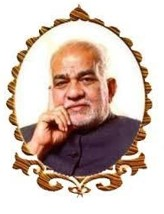
\includegraphics[width=40pt,height=60pt]{bvraju.png}}
\end{picture}}
\huge \textbf{THANK YOU}

\end{center}

\end{frame}

\end{document}